\section{Object-Oriented Design}
\subsection{Objekt Orientierte Grundlagen}
\subsubsection{Beispiel}
Die Grundlagen für \gls{OOP} werden in dem Kurs besprochen. Es soll dabei darum gehen, die Logik hinter den Prinzipen von \gls{OOP} zu verstehen. \\

Es wird versucht die Vorteile zu beschreiben und die Abwegung zwischen verschiedenen Konzepten wie Funktionales-Programmierung aufzuzeigen. \\

Ein kurzes Einführungsbeispiel ist das Kuchen-Backen. Wir können das Backen eines Kuchen als Abfolge verschiedener Prozesse beschreiben, welches zu dem Resultat, einen fertiger Kuchen, führt. Beschreiben wir jedoch den Backvorgang mit \gls{OOP}, dann werden die verschiedenen Gerätschaften beschrieben, mit dem was man mit ihnen tun kann. 
\begin{figure}[H]
	\centering
	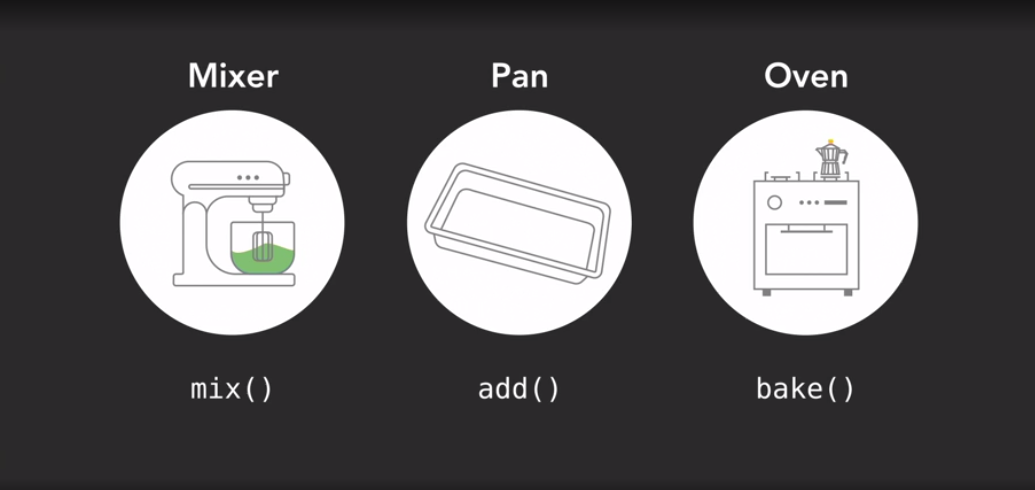
\includegraphics[scale = 0.3]{attachment/chapter_2/Scc002}
	\caption{}
	\label{fig:Scc002}
\end{figure}
\subsubsection{Objekte}
Es wird zuerst ein \textbf{Objekt} beschrieben. Diese kann verschiedenen \textbf{Attribute} besitzen. Oft wird für Attribute auch andere Begrifflichkeiten verwendet:
\begin{align}
	\text{Attribute}\cong \text{Eigenschaften, Status, Variable, Daten etc}\footnote{Das Symbole hat die Bedeutung das die Begriffe ähnlich Struktur aufweisen. In der Geometrie verwendet man nur $\sim$, um gleiche Struktur, aber nicht zwangläufige Größe, auszuweisen. In Algebra verwendet man $\cong$, um \textit{isomorphe} Gebilde auszuweisen: Z. B.: $G\cong H$.}
\end{align}
Im Abstraktenraum sprechen wir von Objekte die Attribute besitzen und mit denen man \textbf{Methoden} vollziehen kann. Auch hier werden oft verschiedenen Begrifflichkeiten verwendet:
\begin{align}
	\text{Methoden}\cong \text{Operationen, Funktionen etc.}
\end{align}Eine Methode ist dabei nur verwenbar von einem Objekt der zugehören Klasse, in welcher die Mehtode definiert wurde. Zwei Objekte vom Typ Konto können wir folgt aussehen:
\begin{figure}[H]
	\centering
	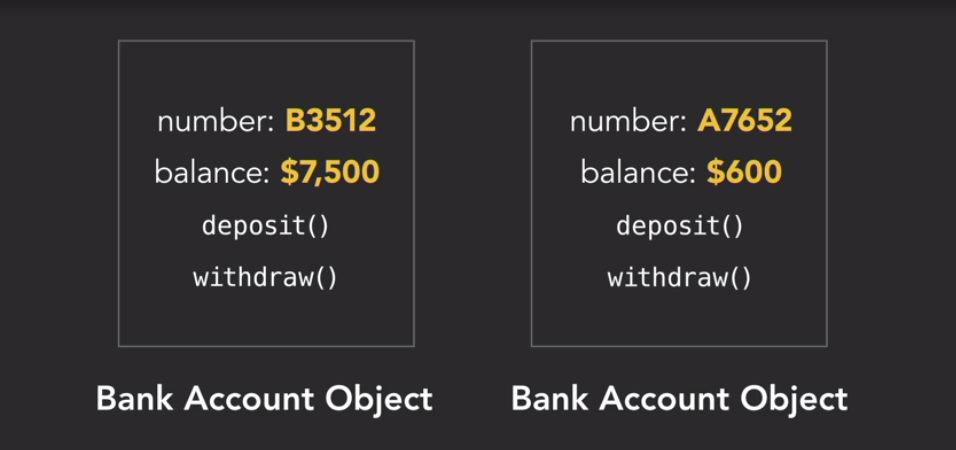
\includegraphics[scale = 0.3]{attachment/chapter_2/Scc003}
	\caption{}
	\label{fig:Scc003}
\end{figure}
Auf das Objekte Bankkonto mit der Nummer $B3512$ können wir die Operation $°deposit()$ ausführen. Dies gilt für alle Bankkonten.

\subsubsection{Klassen}
Die Blaupausen für die Objekte sind die \textbf{Klassen}. Eine Klasse enthält alle Bestandteile für ein Objekte. Ein Objekt wird erst durch eine Klasse erstellt, somit kann eine Klasse mehrere Objekte besitzen. Die Klasse besitzt einen Name:
\begin{align}
	\text{Typ}\cong \text{Name}
\end{align}
und Attribute (Properties) sowie Methoden (Operations)
\begin{figure}[H]
	\centering
	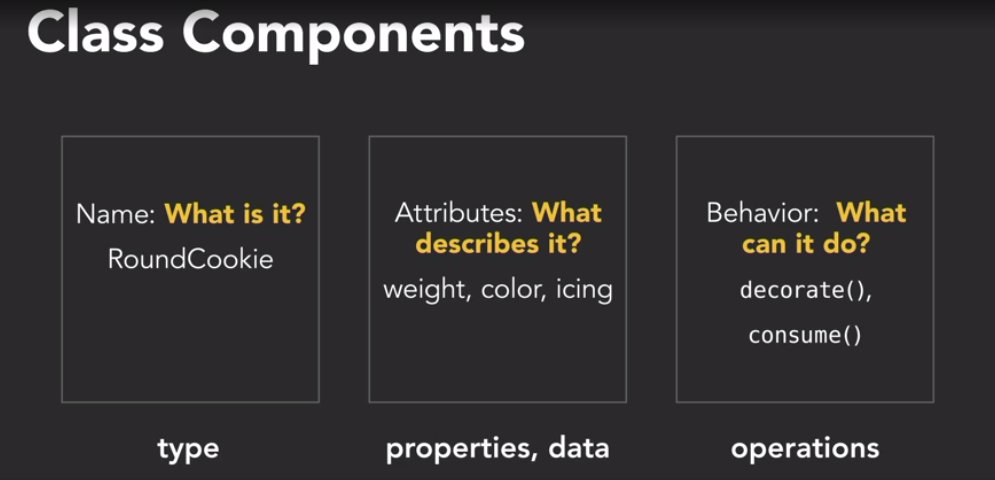
\includegraphics[scale = 0.3]{attachment/chapter_2/Scc004}
	%	\caption{}
	\label{fig:Scc004}
\end{figure}
Eine Klasse wird meist in kompakterer Schreibweise geschrieben:
\begin{figure}[H]
	\centering
	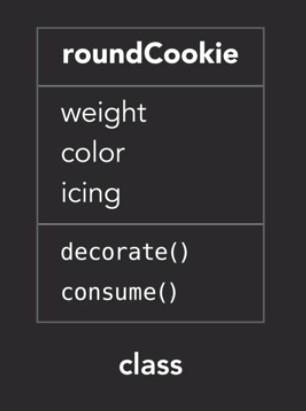
\includegraphics[scale = 0.3]{attachment/chapter_2/Scc006}
	\caption{}
	\label{fig:Scc001}
\end{figure}
Wird ein Objekt erzeugt, so nennt man den Vorgang \textbf{Instanzierung}. Ein Objekt wird auch manchmal \textbf{Instanz} genannt.
\begin{figure}[H]
	\centering
	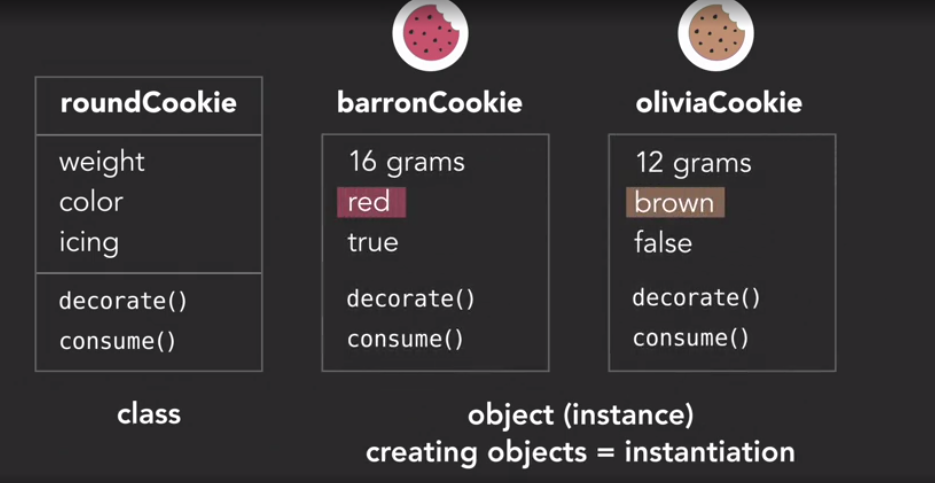
\includegraphics[scale = 0.3]{attachment/chapter_2/Scc005}
	\caption{}
	\label{fig:Scc005}
\end{figure} Die verschiedenen Sprachen habe bereit verschiedene Classen definiert. So zum Beispiel ist ein String, Boolen oder andere Datentypen Classen in den verschiedenen Sprachen. Diese Klassen werden zu \textbf{Bibliotheken} zusammengefasst.
\begin{figure}[H]
	\centering
	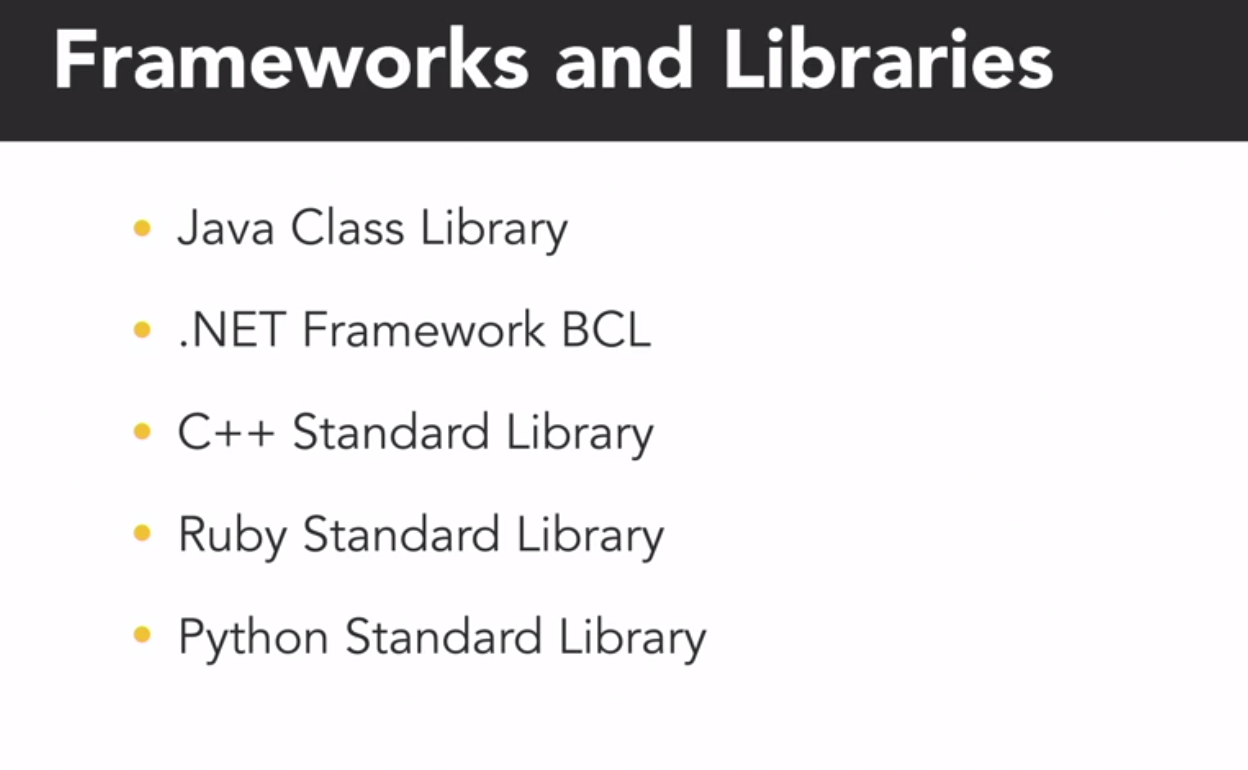
\includegraphics[scale = 0.2]{attachment/chapter_2/Scc007}
	\caption{}
	\label{fig:Scc007}
\end{figure}
\subsubsection{Abstraction, Encapculation, Inheritance, Polymorphismen}
\paragraph{Abstraction} Zum Beschreiben einer Klasse werden nur die wichtigsten Informationen benötigt und die in der einfachsten Form.
\paragraph{Encapculation}
Wir ein Objekt erstellt (instanziert), dann werden die Attribute definiert. Wollen wir aber auf die Attribute zugreifen, so wird der Zugang nur mit Hilfe von Methoden erlaubt. Das bedeutet, soll das Attribute geändert werden, so muss die dafür definierte Methode aufgerufen werden. \\

In dem Beispiel wollen wir ein Keks aus dem Objekt Keksdose entnehmen, dafür wird jedoch die Methoden $requestCokie()$:
\begin{figure}[H]
	\centering
	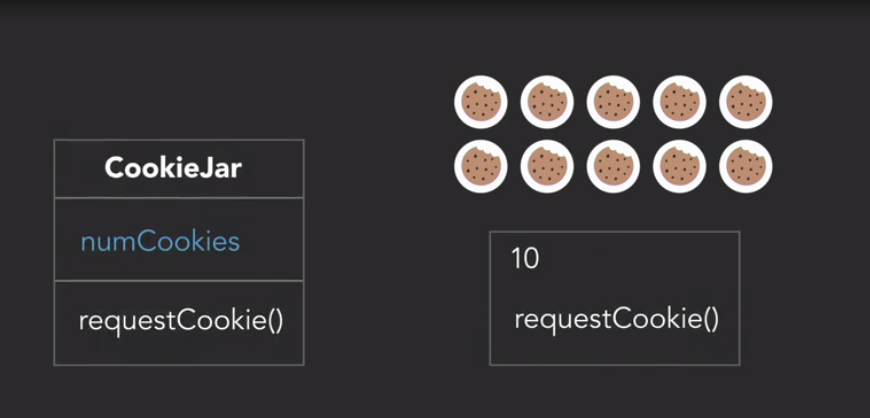
\includegraphics[scale = 0.3]{attachment/chapter_2/Scc008}
	\caption{}
	\label{fig:Scc008}
\end{figure}
Im Code wird dies durch den Ausdruck \textbf{private} hervorgerufen.  
\begin{lstlisting}[style=C++]
	class Account {
		private int account_number;
		private int account_balance;
		
		public void showData() {
			//code to show data 
		}
		
		public void deposit(int a) {
			if (a < 0) {
				//show error 
			} else
			account_balance = account_balance + a;
		}
	}
\end{lstlisting}
Eine Variable kann somit nicht außerhalb der Klasse aufgerufen oder verändert werden. Die Variable ist nur in der Klasse zugänglich. Wollten wir zum Beispiel einen ein Konto aufrufen und einen negative Betrag von $100$ Euro eintrag, würde dies nicht gehen.
\begin{lstlisting}[style=C++]
	Account a = new Account();
	a.account_number = -100;
\end{lstlisting}
Diese Operation könnte somit nicht ausgeführt werden, weil die Variable nicht außerhalb der Klasse verändert werden kann, sondern nur folgendes geht:
\begin{lstlisting}[style=C++]
	Account a = new Account();
	a.deposit(-100);
\end{lstlisting}
Der gesamte Code kann so als Kapsel verstanden werden.
\paragraph{Inheritance}
Die \textbf{Vererbung} von Klassen-Komponenten ist eine sinnvolle Funktion, um weitere Abstraktionsebenen zu erlauben:
\begin{figure}[H]
	\centering
	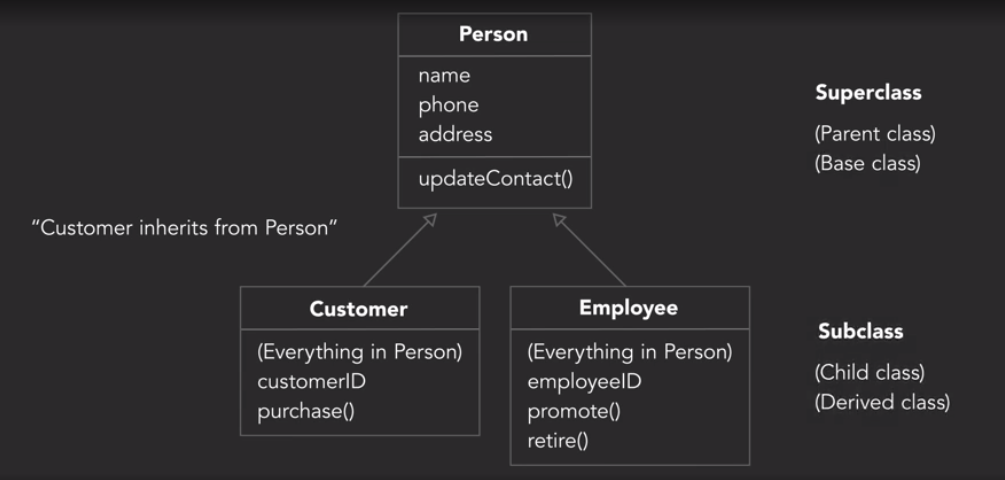
\includegraphics[scale = 0.3]{attachment/chapter_2/Scc010}
	\caption{}
	\label{fig:Scc010}
\end{figure}

Eine Klasse kann auch von mehreren \textbf{Superklassen} eine Vererbung erhalten:
\begin{figure}[H]
	\centering
	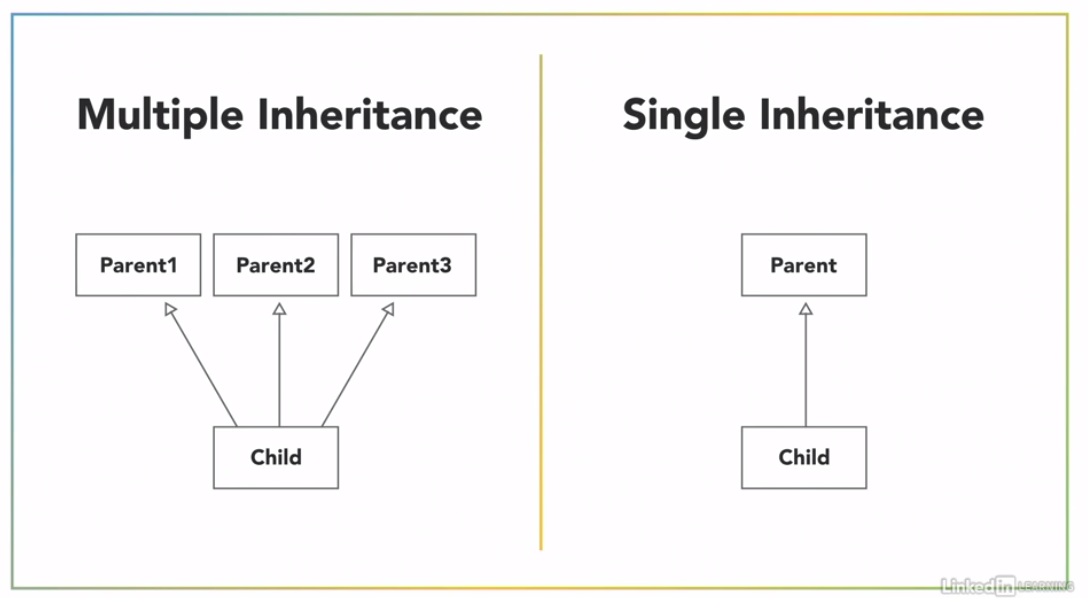
\includegraphics[scale = 0.2]{attachment/chapter_2/Scc011}
	\caption{}
	\label{fig:Scc011}
\end{figure}
\begin{lstlisting}[style=C++]
	Class A(...);      //Base class
	Class B : public A(...);   //B derived from A
	Class C : public B(...);   //C derived from B
\end{lstlisting}

\paragraph{Polymorphism}
Hier wird zwischen \textbf{Statischer} und \textbf{Dynamsicher Polymorphism} unterschied. Wie diese direkt unterschieden werden, hängt von vom Complierprozess ab. Zu jeder der beiden Kategorien lässt sich aber besondere Methode definieren:
\begin{itemize}
	\item Method Overload: Mit Hilfe dieses Prinzip können verschiedene Methoden mit der gleichen Signatur oder Namen definiert werden. Es muss aber möglich sein, Anhand der Inputanzahl oder Typen die Methoden zu differenzieren. 
	\begin{lstlisting}[style=C++]
		void sum (int a , int b);
		void sum (int a , int b, int c);
		void sum (float a, double b);
	\end{lstlisting}
	\item Method Overriding: Soll eine Klasse abgeleitet von einer Superklasse werden, so kann es sein, das nicht alle Methoden genau so verwendet werden sollten. Damit aber nicht die ganze Klasse neu aufgesetzt werden muss, schreibt man nur die Methode um, die anzupassen ist.
	\begin{lstlisting}[style=C++]
		class X{
			public int sum(){
				// some code
			}
		}
		
		class Y extends X{
			public int sum(){
				//overridden method
				//signature is same
			}
		}
	\end{lstlisting}
\end{itemize}
\subsection{Class Diagramm}
\subsubsection{Creating Class Diagramm}
In dem UML Diagramm definieren wir die Variablen/ Attribute zuerst. Hinter dem Doppelpunkt definieren wir den Typ der Variablen und mit mit dem Gleichheitszeichen definieren wir den \textit{Defaultvalue}.\\
\begin{figure}[H]
	\centering
	\begin{tikzpicture}
		\begin{class}[text width=8cm]{ClassName}{0,0}
			\attribute{callSign\textcolor{blue}{: String} =$"$Excellent$"$ }
			\attribute{shieldActive\textcolor{blue}{: Bollean}}
			\attribute{position\textcolor{blue}{: Coordinate}}
			\operation{Methoden}
		\end{class}
	\end{tikzpicture}
\end{figure} Für die Methoden werden meistens Verben in ersten Teil der Bezeichnung für eine Methode verwendet. 
\begin{figure}[H]
	\centering
	\begin{tikzpicture}
		\begin{class}[text width=8cm]{Spaceship}{0,0}
			\attribute{callSign\textcolor{blue}{: String} =$"$Excellent$"$ }
			\attribute{shieldActive\textcolor{blue}{: Bollean}}
			\attribute{position\textcolor{blue}{: Coordinate}}
			\operation{getPosition\textcolor{blue}{()}: Coordinate}
			\operation{setPosition\textcolor{blue}{(integer)}: Coordinate}
			\operation{move\textcolor{blue}{()}: Coodinate}
			\operation{lowerShield\textcolor{blue}{(integer, string)}: Boolean}
		\end{class}
	\end{tikzpicture}
\end{figure} In der Klammer werden die Inputvariablen definiert, die die Methode benötigt. Weiter wird auch hier der Wiedergabetyp, hinter dem Doppelpunkt, definiert.\\

Um \textbf{Private} Klassifizierung in der Klasse zu definieren, werden \textbf{Plus} und \textbf{Minus} genutzt. Ein Plus signalisert, dass das Attribute oder Methode \textbf{public} ist und ein Minus, dass das Attribute oder die Methode \textbf{private} ist.

\begin{figure}[H]
	\centering
	\begin{tikzpicture}
		\begin{class}[text width=8cm]{Spaceship}{0,0}
			\attribute{\textcolor{blue}{+} callSign: String =$"$Excellent$"$ }
			\attribute{\textcolor{blue}{-} shieldActive: Bollean}
			\attribute{\textcolor{blue}{-} position: Coordinate}
			\operation{\textcolor{blue}{+} getPosition(): Coordinate}
			\operation{\textcolor{blue}{-} setPosition(integer): Coordinate}
			\operation{\textcolor{blue}{+} move(): Coodinate}
			\operation{\textcolor{blue}{+} lowerShield(integer, string): Boolean}
		\end{class}
	\end{tikzpicture}
\end{figure} 
\subsubsection{Construktor}
Ein \textbf{Konstruktor} ist eine Methode, welche beim erzeugen der Klasse aufgerufen wird.
Wollen wir ein Objekt erzeugen (instanzieren), verwenden wir
\begin{lstlisting}[style=C++]
	class X{
		public int sum(){
			// some code
		}
	}
	
	X myX = new X();
\end{lstlisting}
Damit nicht die Defaultvalues für die Attribute verwendet werden, sondern wie für $callSign = "Excellent"$, wird der Konstruktor verwendet.
\begin{figure}[H]
	\centering
	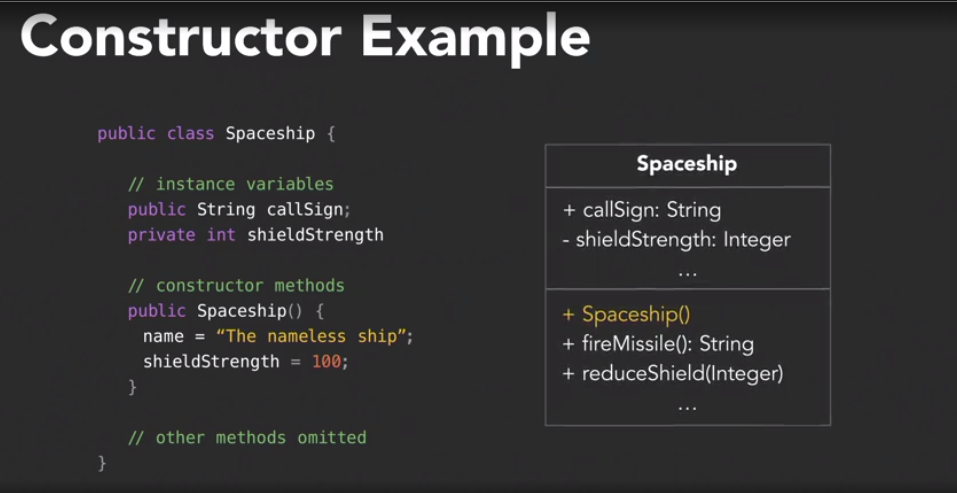
\includegraphics[scale = 0.3]{attachment/chapter_2/Scc012}
	\caption{}
	\label{fig:Scc012}
\end{figure}
Hinweis: Es soll 
\begin{lstlisting}[style=C++]
	public Spaceship() {
		callSign = "The nameless ship";
		NOT name
		shieldStrength = 100;
	}
\end{lstlisting}
heißen. Es können durch die Fähigkeit von \textit{Overloading} mehrer \textit{Konstruktoren} erstellt werden. Diese müssen sich jedoch in ihren Inputvariablen unterscheiden lassen:

\begin{lstlisting}[style=C++]
	public class Spaceship {
		// instance variables
		public String callSign;
		private int shieldStrenght;
		
		// construktor
		public Spaceship() {
			callSign = "The nameless ship";
			shieldStrength = 100;
		}
		
		// overloading construktor
		public Spaceship(String name) {
			callSign = name
			shieldStrength = 200;
			
			// other methods ommitted
		}	
\end{lstlisting}

Instanziert man das Objekt, so folgt, dass man verschieden \textit{Konstruktoren} aufrufen kann.
\begin{lstlisting}[style=C++]
Spaceship yourShip = new Spaceship(); // Erzeugt das "Default" Objekt
Spaceship myShip = new Spaceship("Enterprise"); // Ruft den Overload Construktor auf.
\end{lstlisting}
\subsubsection{Destruktor}
Solle in Objekt gelöscht werden, so verwendet man den Destruktor.

\subsubsection{Static / Instanz Variable/ Methode}
Es gibt zwei Arten von Variable, die \textbf{Instanz Varialben} und die \textbf{Statischen Variablen}, in einer Klasse. 
\begin{description}
\item[Instanz Variable] Dies Form der Variable wir für jedes Objekt in einer Klasse angelegt. Erzeugen wir 3 Objekte in einer Klasse, so erzeugen wir auch 3 \textit{Instanzen Variablen}, wenn diese in der Klasse angelegt wurden. 
\begin{lstlisting}[style=C++]
	public public class Spaceship {
		// Instanz Variable
		public String callSign;
		private int shieldStrength;
		// [...]
	}
	
	// Create two objects
	Spaceship ship1 = new Spaceship();
	Spaceship ship2 = new Spaceship();
\end{lstlisting}
Soll die zugängliche Variable $callSign$ geändert werden, so wird das Objekt und dann die \textit{Instanz Variable} aufgerufen:
\begin{lstlisting}[style=C++]
	ship1.callSign = "Excalibur";
\end{lstlisting}
\item[Static Variable] Die Form der Variablen ist dann nötig, wenn Variablen für mehrer Objekte definiert werden sollen, diese aber nicht für jedes einzelne Objekt geändert werden können. Dies sind mit Globalen Variablen vergleichbar, nur dass sie nicht außerhalb der Klasse existieren. Ändert man eine \textit{statische Variable}, so ändert man den Wert für jedes Objekt der zugehörigen Klasse.
\begin{lstlisting}[style=C++]
public public class Spaceship {
// Static variables
public static float toughness;
//[...]
\end{lstlisting}
Soll der Wert der zugänglichen Variable, $toughness$ geändert werden, wir die Klassen NICHT ein bestimmtes Objekt aufgerufen.
\begin{lstlisting}[style=C++]
Spaceship.toughness = 0.85; // In jeder Klasse wird der Wert angepasst.
\end{lstlisting}
\item[Static Method] Aufbauend auf dem Prinzip von \textit{Statischen Variablen} können \textbf{Static Methods} nur von der Klasse aufgerufen werden. Das Grundprinzip ist, dass auch Statische Variablen nur über Statische Methoden aufgerufen und verändert werden. Ein Konstruktor kann so, zwar eine Initalisierung der Instanzvariablen erzeugen, aber für weitere Änderungen ist es ratsam, die Methoden zu nutzen, um Variablen zu ändern. 
\begin{lstlisting}[style=C++]
public public class Spaceship {
	// Static variables
	public static float toughness;
	// [...]
	public static increasDifficulty(float t){
		toughness += t
	}
\end{lstlisting}
Eine \textit{Static Method} kann nur eine \textit{Static Variable} verändern und vom \textit{Objekt} aufgerufen werden.
\begin{lstlisting}[style=C++]
	Spaceship.increaseDifficulty(0.2); // In jeder Klasse wird der Wert um 0,2 erhöht,
	// wenn die Initalisierung von 0.8 erfolgreich war.
\end{lstlisting}
\item[Static Notierung] In dem UML Diagramm werden statische Objekte mit einem Unterschrich ausgewiesen.
\begin{figure}[H]
	\centering
	\begin{tikzpicture}
		\begin{class}[text width=8cm]{Spaceship}{0,0}
			\attribute{\textcolor{blue}{+} callSign: String =$"$Excellent$"$ }
			\attribute{\textcolor{blue}{-} shieldActive: Bollean}
			\attribute{\textcolor{blue}{-} position: Coordinate}
			\attribute{\underline{\textcolor{blue}{+} toughness: float}}
			\operation{\textcolor{blue}{+} getPosition(): Coordinate}
			\operation{\textcolor{blue}{-} setPosition(integer): Coordinate}
			\operation{\textcolor{blue}{+} move(): Coodinate}
			\operation{\textcolor{blue}{+} lowerShield(integer, string): Boolean}
			\operation{\underline{\textcolor{blue}{+} increaseDifficulty(float)}}
		\end{class}
	\end{tikzpicture}
\end{figure} 
\end{description}
\subsection{Inheritance and Composition}
Es ist nicht ratsam, nach \textit{Vererbung} zu suchen und verschiedenen Ebenen von Beziehungen zu erstellen. \textbf{Inheritance} $"$ will reveal is self$"$. \textbf{Overriding} ist ein essentieller Teil der Vererbung. Ebenso ist es möglich weitere Methoden einer Klasse zuzufügen. \\

In $C++$ wird der Doppelpunkt verwendet, um eine Klasse einer Superklasse zuzuweisen:
\begin{lstlisting}[style=C++]
public class CargoShuttel : Spaceship {
	\\ CargoShuttel inherent all from Spaceship
}
\end{lstlisting}
Beim Beschreiben der hergeleiteten Klasse, wird von Sprache zu Sprache unterschied, welche Syntax zu verwenden ist. In Java wird der Prefix \textbf{super}, in $C\#$ \textbf{base}, verwendet. 
\textcolor{blue}{Hinweis:} In einer Klasse, kann auch eine Methode beschrieben werden, die ein Objekt der Klasse intanziert.\\

Im folgenden Beispiel
\begin{lstlisting}[style=C++]
class left {
	public:
	void foo();
};

class right {
	public:
	void foo();
};

class bottom : public left, public right {
	public:
	void foo()
	{
		//base::foo();// ambiguous
		left::foo();
		right::foo();
		
		// and when foo() is not called for 'this':
		bottom b;
		b.left::foo();  // calls b.foo() from 'left'
		b.right::foo();  // call b.foo() from 'right'
	}
};
\end{lstlisting}
wird der Synatk $::$ benötigt, um auf die Superklasse zu referieren. In C++ kann auch auf zwei Superklassen referiert werden. Andere Klassen verweisen, in der Regel nur auf eine Superklasse. 
\subsubsection{Abstract class/ Methode}
Eine \textbf{Abstrakte Klasse} ist eine Form der Klasse, welche eine Initialiszierung zu lässt. Der Zweck dieser Form ist, dass die Klasse als Super Klasse dient. Dabei kann eine Abstrakte Klasse auch selber eine Subklasse sein, jedoch wird von dieser Ebenen mindestens eine weitere Ebene erschlossen. 
\begin{lstlisting}[style=C++]
public abstract class GraphicObject {
	// declare variables
	// declare nonabstract methods
	abstract void draw();
}
\end{lstlisting}
Eine \textbf{Abstrakte Methode} wird ohne Implementation geschrieben. D. h., hinter $(...)$ wird nur $;$ gesetzt. In der Subklasse wird diese Methode dann implementiert: \textit{Override}. Wird die Methode nicht implementiert, so muss die Sub Klasse auch abstrakt sein.\\

Die Methoden die zu überschreiben sind, werden dann, im Normalfall, als abstrakt dekliniert. Selbst, wenn diese nicht notwendig ist, hilft es, die Intention in dem programmierten Text besser zu vermitteln.
\begin{lstlisting}[style=C++]
abstract class GraphicObject {
	int x, y;
	...
	void moveTo(int newX, int newY) {
		...
	}
	abstract void draw();
	abstract void resize();
}

class Circle extends GraphicObject {
	void draw() {
		// Overriding 
	}
	void resize() {
		// Overriding
	}
}
class Rectangle extends GraphicObject {
	void draw() {
		// Overriding
	}
	void resize() {
		// Overriding
	}
}
\end{lstlisting}
Schlussfolgerung: Eine \textbf{abstract class} ist nur zur Vererbung angelegt. Objekte können auch nicht über diese Klasse intanziert werden.
\subsubsection{Interfaces}
Es gibt einige Unterschied zwischen \textit{Abstract class} und \textbf{Interface}. Auf dem ersten Blick wirken beide jedoch sehr ähnlich. Das Interface wirkt auch wie extreme Variante der Abstrakten Klasse. Die Zielsetzung mit der man die Klassen erstellt, sind aber andere. 
\begin{description}
\item[Abstrakte Klasse] wird verwendet, wenn Klassen verschiedenen Beziehungen miteinander habe und eine Hierachiche Struktur besitzen. Bei $C++$ können Klassen von mehren Superklassen die Eigenschaften erhalten, bei den meisten anderen Sprachen jedoch nicht - Hierachische Struktur. 
\item[Interface] wird verwendet, wenn Fähigkeiten übertragen werden sollen. Die Fähigkeit $move()$ und $draw()$ lässt sich besser jeweiligen Interface Klassen zuordnen, als eine hierachische Abstrakte Klasse zu erzeugen. 
\end{description}
\begin{figure}[H]
\centering
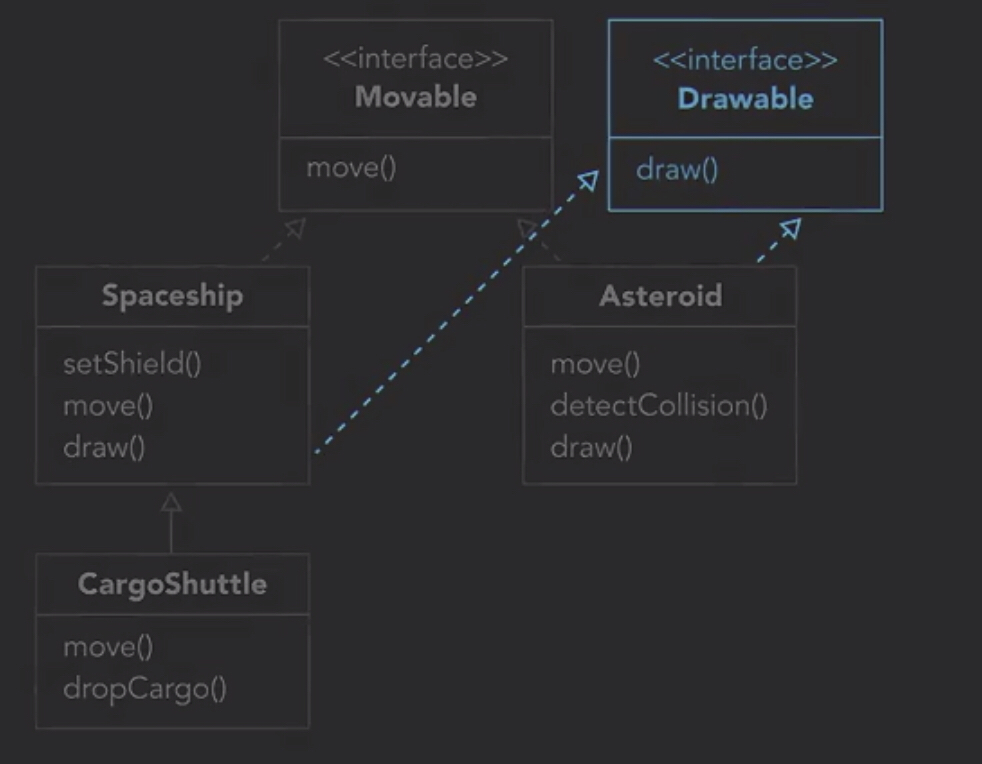
\includegraphics[scale = 0.3]{attachment/chapter_2/Scc013}
\caption{}
\label{fig:Scc013}
\end{figure}
In dem UML Diagramm werden Interface mit gepunkteten Linien gezeignet.\\

Eigenschaften
\begin{itemize}
\item Alle Variablen und Methoden sind \textcolor{blue}{public, static}. $\neq$ In einer Abstrakten Klasse kann eine Methode abstrakt sein. 
\begin{lstlisting}[style=C++]
	interface Moveable {
		// methode signate
		void move(int x, int y);
		
		class X implements Moveable {
			// Implementation for interface method
			public void move(int x, int y){
				// Implementation code
			}
			// Additional methodes
		}
	\end{lstlisting}
	\item Alle Methoden besitzen keine Implementation. 
	\item Keine Methode muss mit public oder private deklariert werden. 
\end{itemize}

\subsubsection{Aggregation / Composition}
Diese beiden Relationen beziehen sich nicht so sehr auf eine besondere Syntax, sondern auf die Gestaltung des Codes.
\begin{figure}[H]
	\centering
	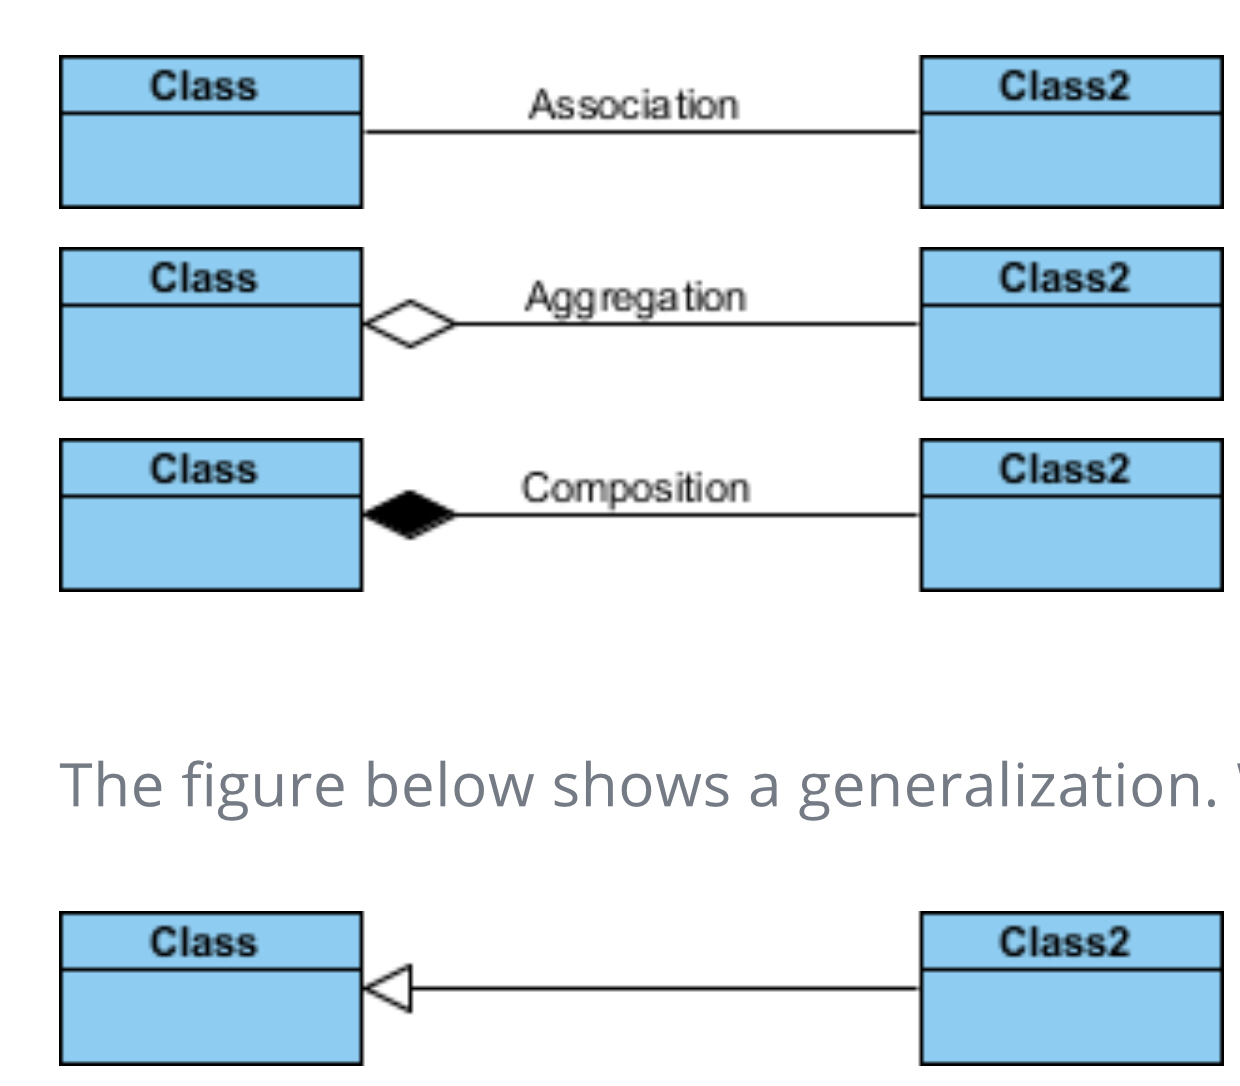
\includegraphics[scale = 0.3]{attachment/chapter_2/Scc014}
	\caption{}
	\label{fig:Scc014}
\end{figure}
\begin{itemize}
	\item Die Relation \textbf{Aggregation} wird so verstanden, dass ein Subobjekt, in einer Gruppenabhängigkeit einbezogen wird. Löst sich diese jedoch auf, bleibt das erzeugt Objekt erhalten.
	\item Die Realation \textbf{Composition} wird so verstanden, dass ein Subobjekt, in einer Gruppenabhängigkeit einbezogen wird. Löst sich diese jedoch auf, so hört das erzeugt Objekt auf zu existieren. 
\end{itemize} 
Zum Beispiel: Ein Spaceship kann teil einer Field sein. Verschwindet die Flied, so verschwindet das Spaceship nicht zwangsläufigerweise. 
\begin{figure}[H]
	\centering
	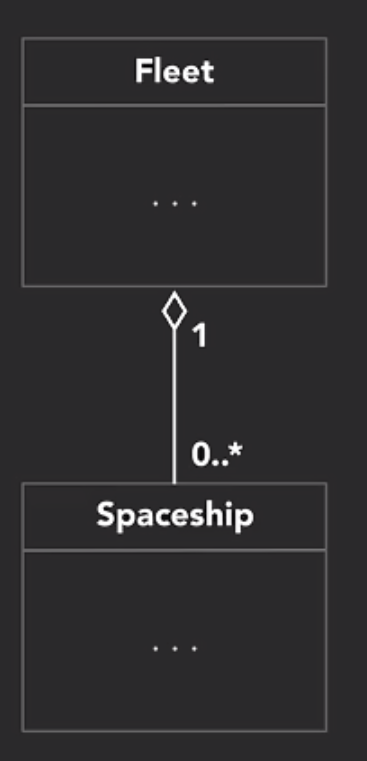
\includegraphics[scale = 0.2]{attachment/chapter_2/Scc015}
	\caption{}
	\label{fig:Scc015}
\end{figure}
Zum Beispiel: Ein Auto besteht aus einem Motor und Reifen. Wenn das Auto nicht mehr ist, wird der Motor nicht mehr benötigt.
\begin{figure}[H]
	\centering
	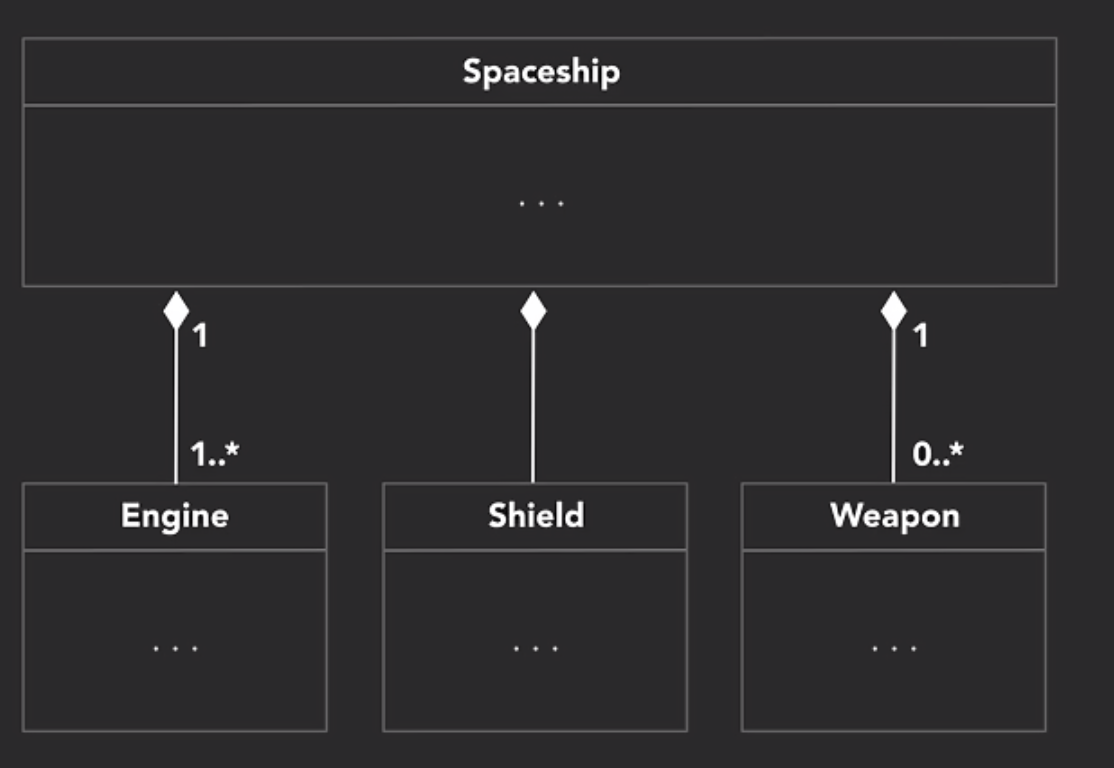
\includegraphics[scale = 0.2]{attachment/chapter_2/Scc016}
	\caption{}
	\label{fig:Scc016}
\end{figure}
\textbf{Hinweis} Mit Hilfe der UML Beziehungsanalyse soll die Programmiererin erkennen, welche Objekte mit einem \textit{Destruktor} gelöscht werden müssen und welche nicht. 
\subsubsection{Zusammenfassung Relationen}
\begin{figure}[H]
	\centering
	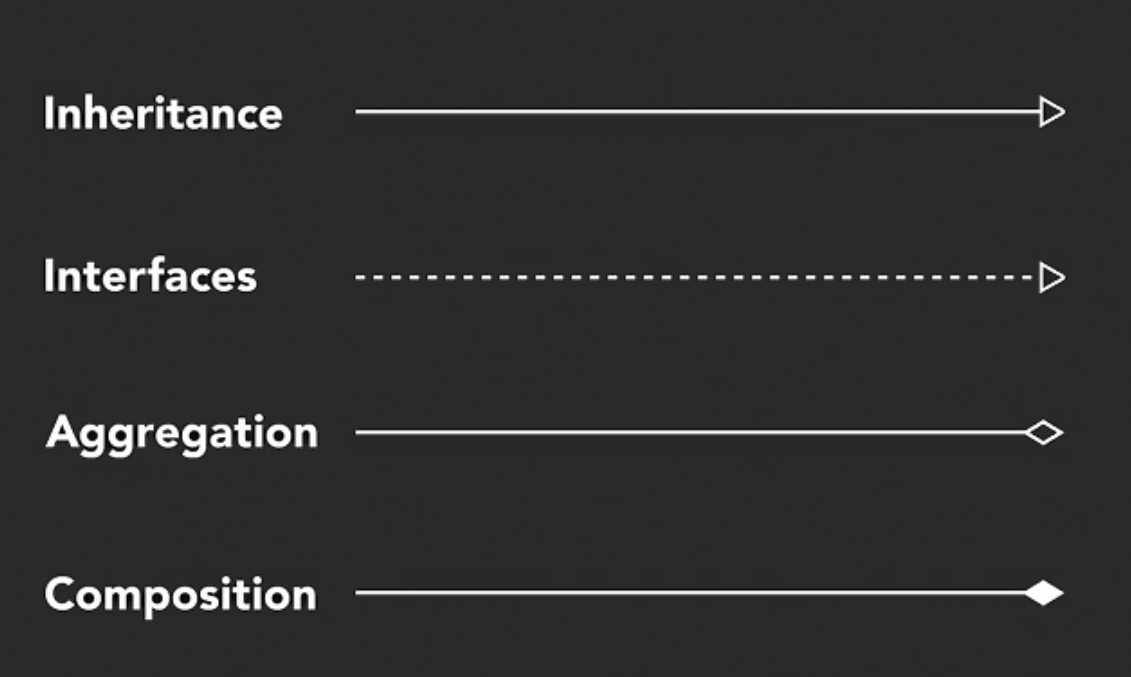
\includegraphics[scale = 0.2]{attachment/chapter_2/Scc017}
	\caption{}
	\label{fig:Scc017}
\end{figure}
\subsection{Software Development}

\begin{figure}[H]
	\centering
	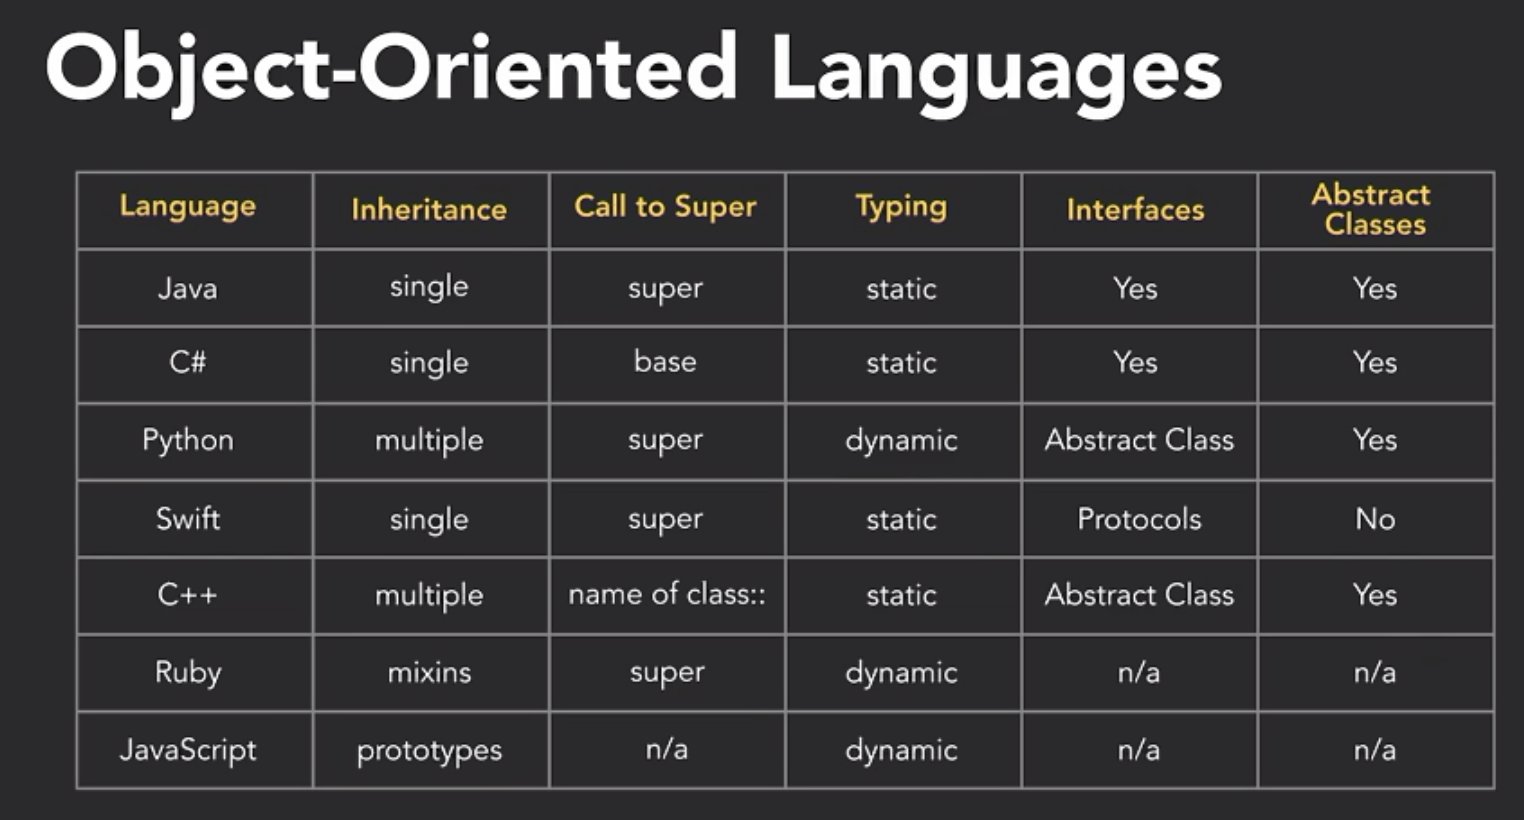
\includegraphics[scale = 0.2]{attachment/chapter_2/Scc018}
	\caption{}
	\label{fig:Scc018}
\end{figure}
Die verschieden Sprachen könnnen unterschiedlich mit den Prinzipien, die wir besprochen haben, umgehen.
\begin{itemize}
	\item Inheritance: Kann eine Klasse vererbt werden. Bei $C++$ können auch mehrere Klassen einer Klasse vererbt werden.
	\item Call to super: Wie lautet die Syntax, um eine Vererbung anzuzeigen.
	\item Typing: ? Das Thema ist noch unklar. Stichphrase: Wie wird kompeliert? Es gibt hierzu Vor- und Nachteil. Zum Beispiel: Bei static languages müssen alle Variablen vom Typ definiert werden, da sie vor dem Ausführen vorliegen. Bei dynamischen Sprachen wird der Typ bei Ausführung erkannt. Dies kann jedoch zu Problemen führen, falls die Erkennung nicht richtig erfolgt. Das Schreiben des Codes ist aber einfacher.
\end{itemize}
